\section{Isothermal Annealing Studies}
\label{sec:annealing}

\begin{itemize}
	\item Annealing, i.e. heating up, during long shutdowns
	\item \SI{80}{\minute} at \SI{60}{\celsius} corresponds to xx at yy or cc at bb
	\item Systematic annealing study for all sensors was beyond the scope of this study, and anyways not possible due to high temperatures / annealing during irradiation
	\item Hence: focus on one illustrative example
	\item \ref{plot:annealing_IV,plot:annealing_current} illustrate the improvement in leakage current for a sensor with minimal additional annealing during irradiation
	\item \ref{plot:annealing_IV}: IV curves lowered especially at high bias voltages beyond full depletion where bulk currents dominate
	\item \ref{plot:annealing_current}: Current at \SI{600}{\volt} reduced by approximately 25$~\%$ for all pads
	\item \ref{plot:annealing_CV} shows a comparison of inverted CV curves after different annealing times, earlier saturation clearly visible, no change in end capacitance (as expected)
	\item \ref{plot:annealing_Vdep}: Depletion voltage estimated (cf. \ref{subsec:QA_Vdep}) reduced sizeably, about 40$~\%$ in case of \SI{200}{\micron}
\end{itemize}

\begin{figure}
	\captionsetup[subfigure]{aboveskip=-1pt,belowskip=-1pt}
	\centering
	\begin{subfigure}[b]{0.49\textwidth}
		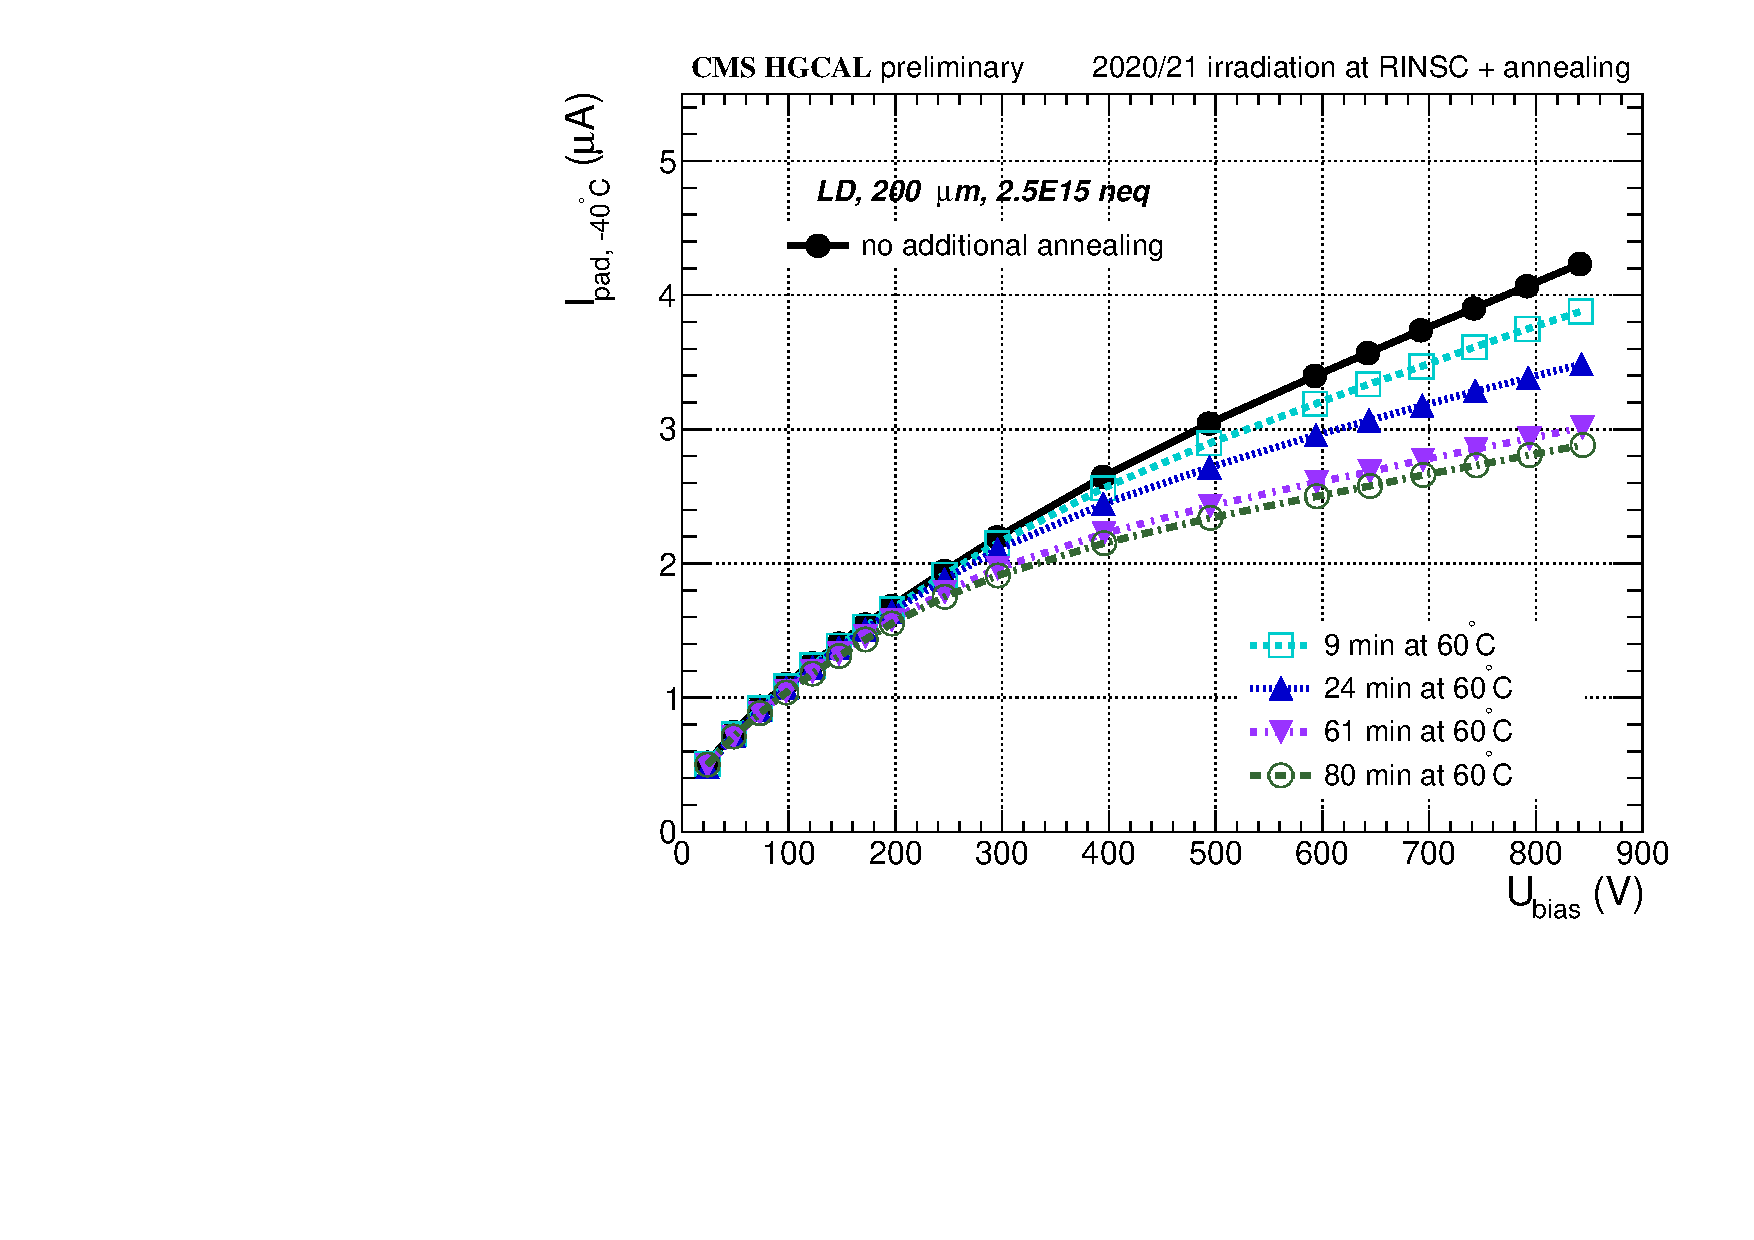
\includegraphics[width=0.999\textwidth]{plots/annealing_iv/annealing_IV_ch24.pdf}
		\subcaption{
		}
		\label{plot:annealing_IV}
	\end{subfigure}
	\hfill
	\begin{subfigure}[b]{0.49\textwidth}
		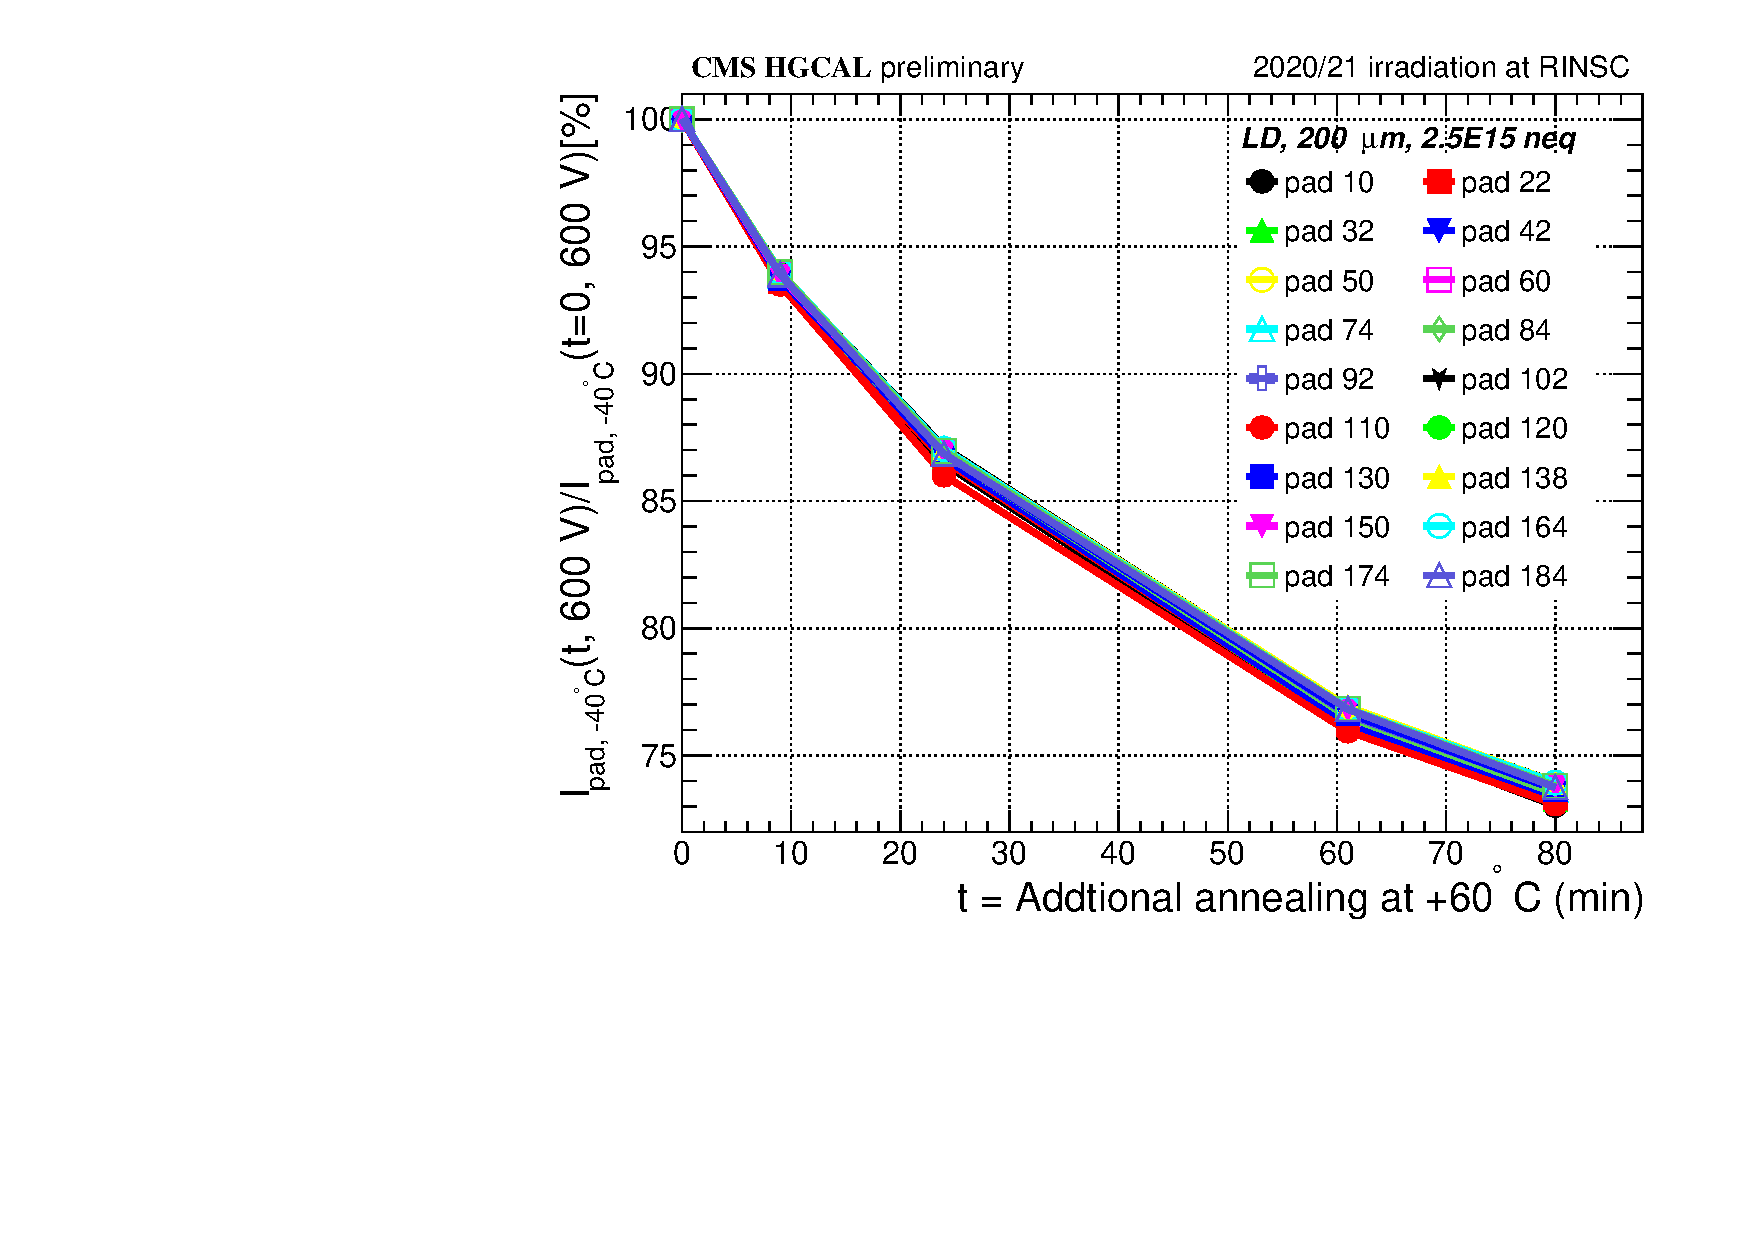
\includegraphics[width=0.999\textwidth]{plots/annealing_iv/annealing_current.pdf}
		\subcaption{
		}
		\label{plot:annealing_current}
	\end{subfigure}
	\caption{
		(a) IV-curves of a representative full hexagonal pad for different annealing scenarios for a \SI{200}{\micro\metre} low-density prototype sensor irradiated to 2.5$~$E15 1-MeV-neutron equivalents/cm$^{2}$.
        (b) Decrease of the per-pad leakage current (interpolated to $U_\text{bias}=\SI{600}{\volt}$) as a function of the additional annealing time at \SI{60}{\celsius} for a subset of full pads.
	}
\end{figure}

\begin{figure}
	\captionsetup[subfigure]{aboveskip=-1pt,belowskip=-1pt}
	\centering
	\begin{subfigure}[b]{0.49\textwidth}
		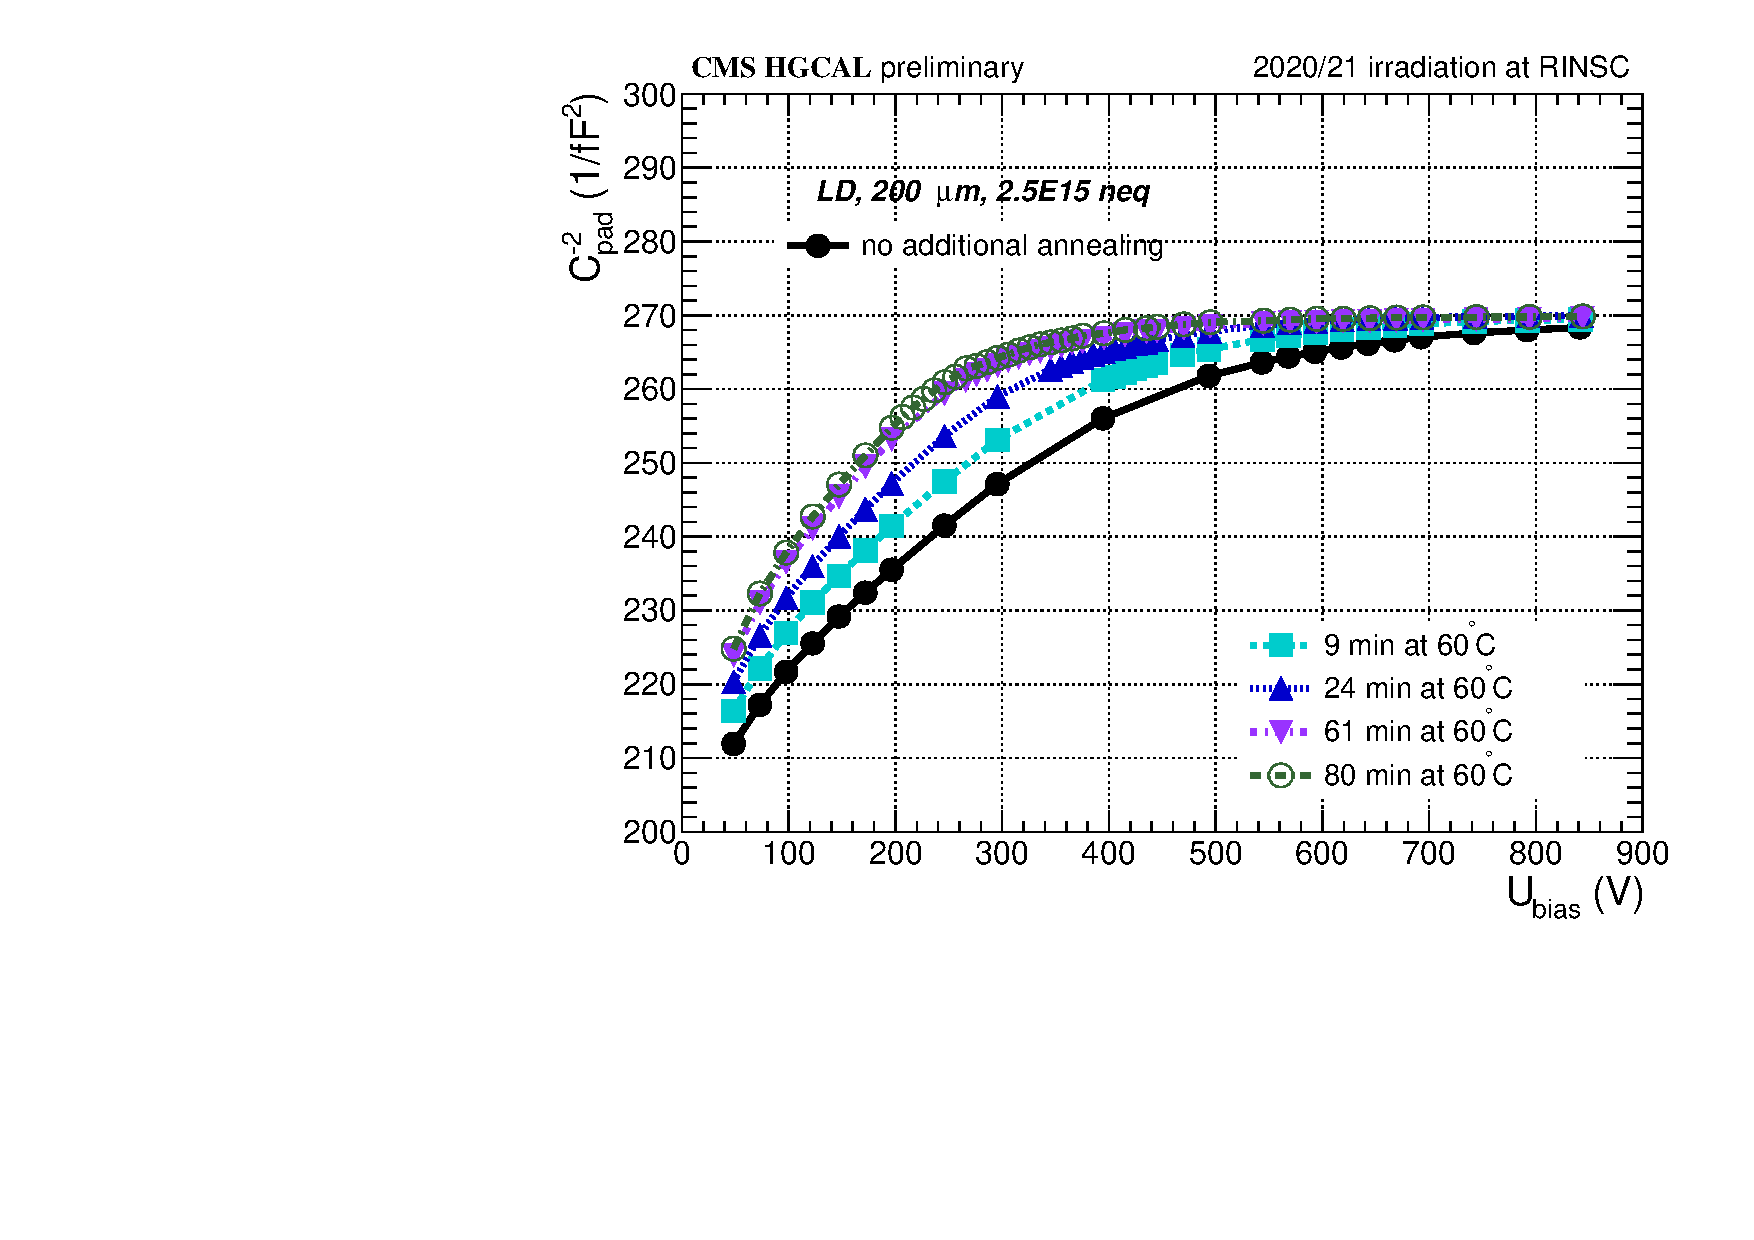
\includegraphics[width=0.999\textwidth]{plots/annealing_Vdep/annealing_CV_ch24.pdf}
		\subcaption{
		}
		\label{plot:annealing_CV}
	\end{subfigure}
	\hfill
	\begin{subfigure}[b]{0.49\textwidth}
		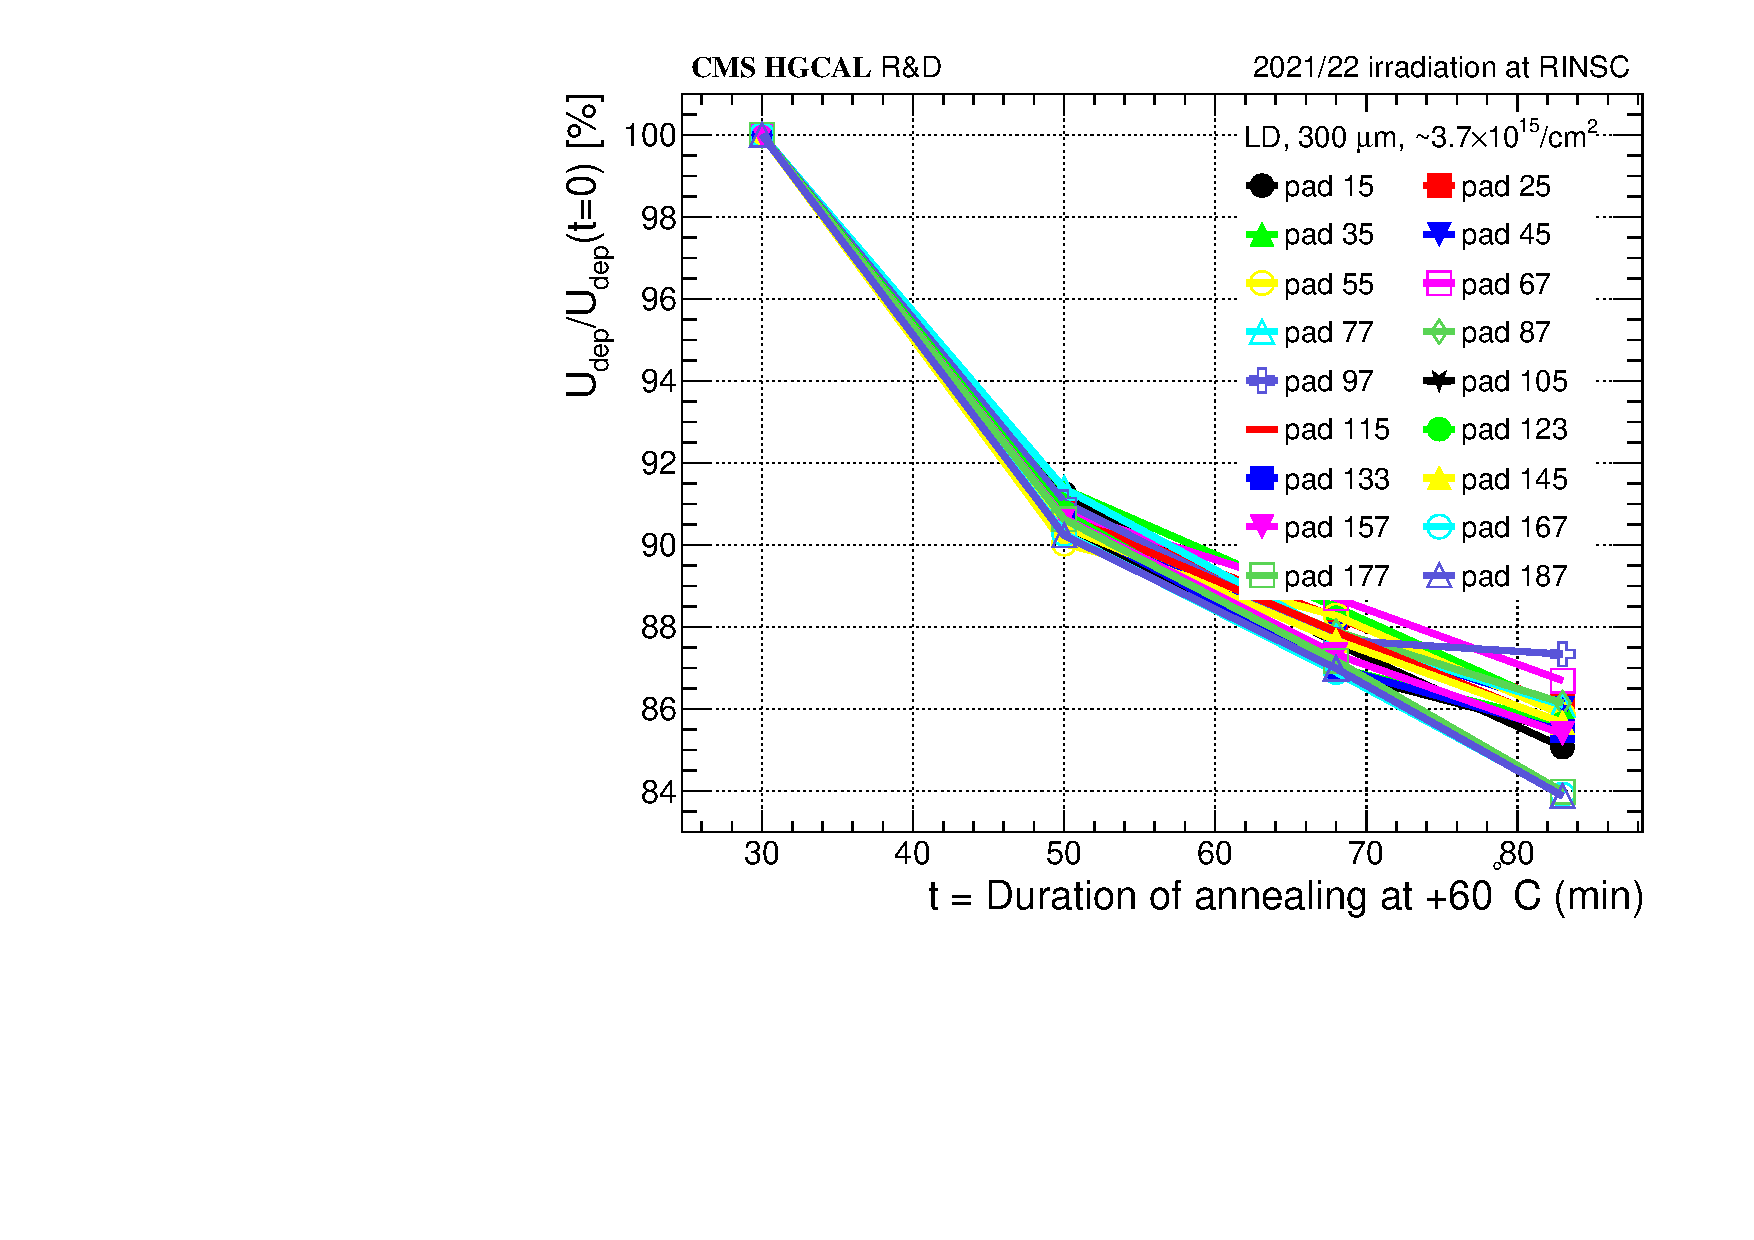
\includegraphics[width=0.999\textwidth]{plots/annealing_Vdep/annealing_Vdep.pdf}
		\subcaption{
		}
		\label{plot:annealing_Vdep}
	\end{subfigure}
	\caption{
		(a) (Inverted) CV-curves of a representative full hexagonal pad for different annealing scenarios for a \SI{200}{\micro\metre} low-density prototype sensor irradiated to 2.5$~$E15 1-MeV-neutron equivalents/cm$^{2}$.
        (b) Decrease of the depletion voltage estimate ($U\text{dep}$) as a function of the additional annealing time at \SI{60}{\celsius} for a subset of full pads.
	}
\end{figure}